\chapter{Theorieteil}

\thispagestyle{standard}
\pagestyle{standard}

\section{Lebenszykluskonzepte}

\begin{quote}
Lebenszykluskonzepte gehen davon aus, dass bestimmte Bezugsobjekte (z.B. Marken, Produkte, Branchen) im Zeitablauf einem gesetzmäßigen Verlauf folgen, der natürlichen Organismen ähnelt \upshape \cite[S. 61]{Bru06}.
\end{quote}

Das Lebenszykluskonzept erhielt in den 1960er Jahren Einzug in die Marketingtheorie und Unternehmenspraxis. Seitdem wurde es auf unterschiedliche Untersuchungsobjekte angewandt. Das Lebenszykluskonzept versucht unter Beobachtung zeitlicher Entwicklungsprozesse entsprechende Grundsatzentscheidungen festzulegen. Der Verlauf des Lebenszykluskonzeptes entspricht einem idealisierten Modell, weshalb es für die Praxis nur bedingt anwendbar ist. Es dient jedoch als Anhaltspunkt bei der Analyse und Prognose von Untersuchungsobjekten. 
Auf Basis eines allgemeinen Nachfragelebenszyklus haben sich im Laufe der Zeit verschiedene Formen des Lebenszykluskonzeptes entwickelt \cite{Bru06}:

\begin{itemize}[noitemsep]
\item Produktlebenszyklus
\item Marktlebenszyklus
\item Technologielebenszyklus
\item Kundenlebenszyklus 
\end{itemize}

Auf die speziell für diese Arbeit wichtigen Produkt- und Technologielebenszyklen wird in den nächsten Kapiteln näher eingegangen.

\subsection{Produktlebenszyklus}

Der Produktlebenszyklus beschreibt die Entwicklung eines Produktes von der Markteinführung bis zum Marktaustritt, gemessen an den Größen Umsatz, Gewinn, und/oder Deckungsbeitrag \cite{Pep99}. 

Wie in Abb. \ref{img:produktlebenszyklus} ersichtlich, wird der Lebenszyklus in fünf Phasen eingeteilt. Die Einführungsphase, Wachstumsphase, Reifephase, Sättigungsphase und Rückgangsphase \cite{Poeschek00}. 

\begin{figure}[h!]
	\centering
	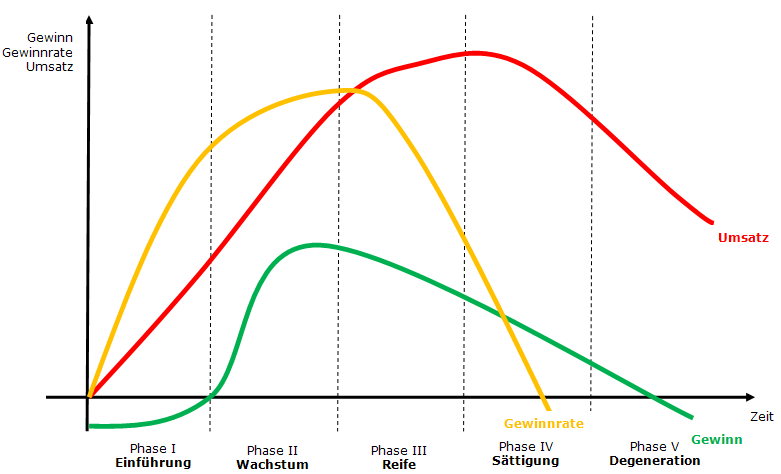
\includegraphics[width=0.6\textwidth]{BilderAllgemein/produktlebenszyklus.png}
	\caption{Einzelnen Phasen des Produktlebenszyklus \cite{Deef09}}
	\label{img:produktlebenszyklus}
\end{figure}

Bei international vermarkteten Produkten kann es vorkommen, dass sich die Produkte abhängig von der Region in unterschiedlichen Phasen befinden. Weiters stellt der Produktlebenszyklus keine genaue Prognose für jedes Produkt dar und kann somit variieren. Im Folgenden werden die einzelnen Phasen beschrieben \cite{Poeschek00}.

\textbf{Einführungsphase}

In der ersten Phase ist der Umsatz noch sehr gering und der Gewinn negativ, da das Produkt erst am Markt eingeführt wurde und hohe Einführungskosten vorhanden sind. Eine steigende Tendenz ist jedoch schon ersichtlich. Gute Werbung und Öffentlichkeitsarbeit sind in dieser Phase unerlässlich und können mitentscheiden, ob das Produkt den Einstieg schafft oder zum Flop wird. Bei Erreichen des Break Even Points ist die Einführungsphase beendet und die Wachstumsphase beginnt \cite{Poeschek00}.

\textbf{Wachstumsphase}

In der Wachstumsphase wurde das Produkt erfolgreich am Markt eingeführt und Umsatz und Absatz steigen stark an. Marktanteile wachsen und Konkurrenten werden auf das Produkt aufmerksam. Es gilt durch Unterstützung von Marketingaktivitäten den Markt mit dem eigenen Produkt weiter zu durchdringen. Weiters sollten in dieser Phase die Herstellungskosten durch das Mengenwachstum gesenkt werden \cite{Poeschek00}.

\textbf{Reifephase}

In der Reifephase hat sich das Produkt so weit am Markt verbreitet, dass das Wachstum stagniert. Sie gilt allgemein als die längste und profitabelste Phase und sollte deshalb so weit als möglich gestreckt werden. Die Verteidigung der Marktposition gegenüber den Konkurrenten ist essentiell. Der Übergang in die Reifephase kann an mehreren Faktoren erkannt werden. Dazu gehört die Zunahme der internationalen Konkurrenz, der Kampf um Marktanteile sowie die Zunahme von Preis- und Serviceorientierung aufgrund der wachsenden Erfahrungen der Unternehmen. Weiters erreicht der Gewinn in dieser Phase seinen Höhepunkt und beginnt wieder zu sinken, wohingegen der Umsatz weiter steigt \cite{Poeschek00}.

\textbf{Sättigungsphase}

Die Sättigungsphase ist dann erreicht, wenn keine zusätzlichen Marktteilnehmer mehr gewonnen werden können. Wie in Abb. \ref{img:saettigung} ersichtlich, muss das Unternehmen an diesem Punkt entscheiden, ob eine Neuorientierung erfolgt, das Produkt aufgegeben wird oder solange weitergeführt wird, wie Gewinne erwirtschaftet werden. Weiters sollten in der Sättigungsphase die Ursachen für den Rückgang der Nachfrage untersucht werden \cite{Poeschek00}.

\begin{figure}[h!]
	\centering
	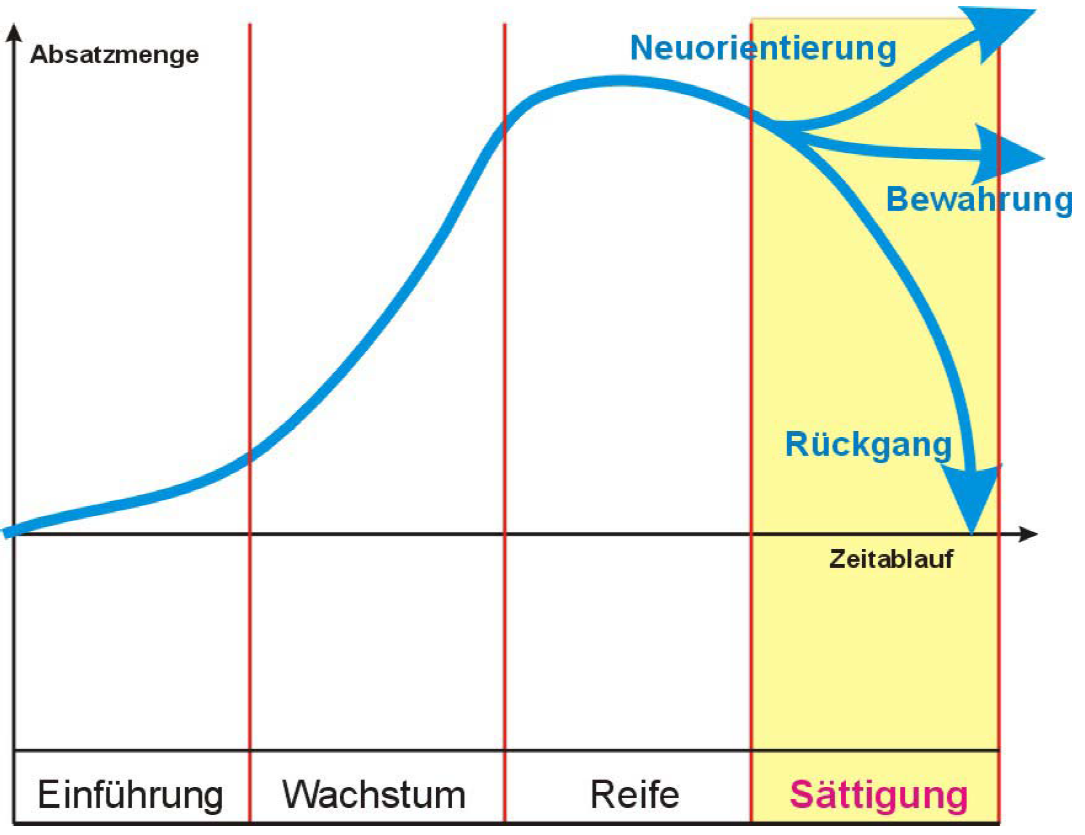
\includegraphics[width=0.45\textwidth]{BilderAllgemein/saettigung.png}
	\caption{Sättigungsphase Entscheidungen \cite{Poeschek00}}
	\label{img:saettigung}
\end{figure}

\textbf{Rückgangsphase}

In der Degeneration beziehungsweise Rückgangsphase schrumpft der Absatzmarkt kontinuierlich und dem Umsatzrückgang kann auch durch gezielte Marketingmaßnahmen nicht entgegengewirkt werden. Wenn vom Unternehmen in der Sättigungsphase keine Neuorientierung erfolgt, ist das Produkt mit Ende dieser Phase "gestorben" \cite{Poeschek00}.

\subsection{Technologielebenszyklus}

Das Modell des Technologielebenszyklus ist Teil des strategischen Innovationsmanagements und dient dazu, die Position einer Technologie in ihrem jeweiligen Lebenszyklus zu finden. Es wird davon ausgegangen, dass der von der Technologie durchlaufene Zyklus von der Nachfrage nach Produkten und Services, welche auf dieser Technologie beruhen, abhängt \cite{Bru06} \cite{Schumann03}.

Im Allgemeinen ist der Technologielebenszyklus ein an den Produktlebenszyklus angepasster idealtypischer Entwicklungsverlauf einer Technologie. Wie in Abb. \ref{img:technologielebenszyklusmodell} ersichtlich ist der Kurvenverlauf s-förmig und kann in die vier Technologiephasen \textbf{Entstehung, Wachstum, Reife und Alter} unterteilt werden \cite{Schumann03}.

\begin{figure}[h!]
	\centering
	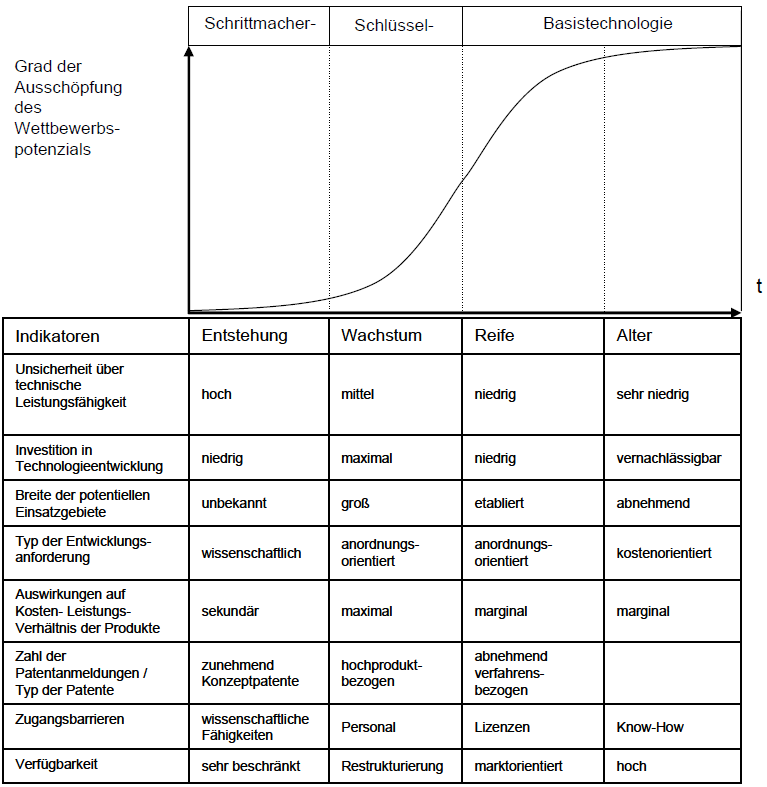
\includegraphics[width=0.8\textwidth]{BilderAllgemein/technologielebenszyklusmodell.PNG}
	\caption{Technologielebenszyklusmodell von Arthur D. Little \cite{Gerpott05}}
	\label{img:technologielebenszyklusmodell}
\end{figure}

Weiters werden drei Technologietypen unterschieden, welche als Schrittmacher- Schlüssel- und Basistechnologie bekannt sind \cite{Schumann03}.

\textbf{Schrittmachertechnologien} sind soeben erst am Markt eingeführt worden und befinden sich am Anfang ihrer Entwicklung. Mit zunehmender Verbreitung werden sie zu Schlüsseltechnologien heranreifen, sofern sie nicht zuvor vom Markt verdrängt werden. \\
Hat die Technologie eine Marktreife erreicht, so wird von \textbf{Schlüsseltechnologien} gesprochen. In dieser Phase existiert noch ein erhebliches Verbesserungspotential und die Möglichkeit für den Aufbau von Wettbewerbsvorteilen. \\
Ab einer gewissen Reife spricht man von \textbf{Basistechnologien}. Aufgrund einer meist bereits großen allgemeinen Verfügbarkeit ist das wettbewerbsstrategische Potential in dieser Phase sehr gering \cite{Bru06} \cite{Schumann03}.

\subsubsection{S-Kurve}

Zum Vergleichen zweier Technologien in Bezug auf ihre Vorteilhaftigkeit wird das Konzept der \textbf{S-Kurve}, siehe Abb. \ref{img:s-kurve}, verwendet \cite{Schumann03}.

\begin{figure}[h!]
	\centering
	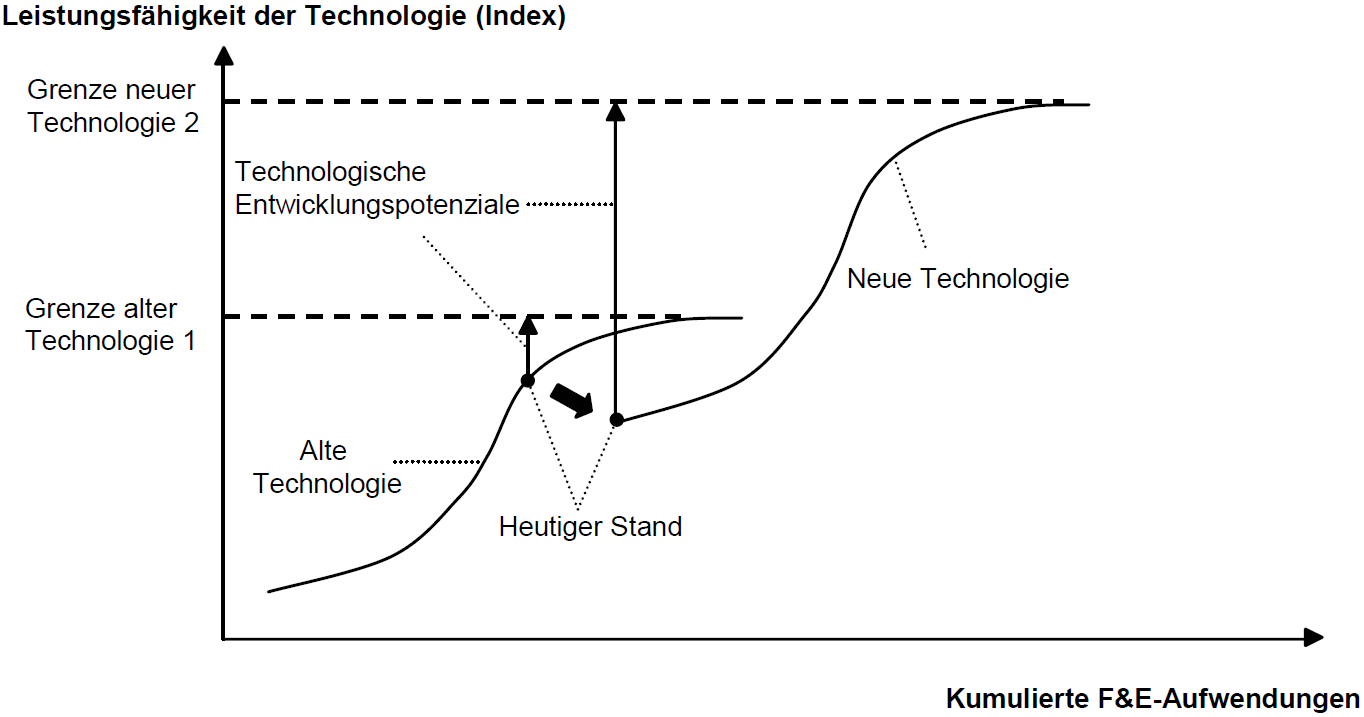
\includegraphics[width=0.9\textwidth]{BilderAllgemein/s-kurve.PNG}
	\caption{S-Kurven Modell von McKinsey \cite{Gerpott05}}
	\label{img:s-kurve}
\end{figure}

Zu Beginn lässt sich die Leistungsfähigkeit mit relativ geringen Investitionen steigern. Mit zunehmender Reife wird das Beibehalten des Leistungszuwachses immer schwerer, wodurch sich ein Wechsel zu einer Technologie mit höherer Leistungsfähigkeit empfiehlt. Die Grenze einer Technologie wird oft durch natürliche Eigenschaften, wie Größe oder Materialeigenschaften, welche nicht mehr gesteigert werden können, bestimmt \cite{Bru06}.

Das Konzept der S-Kurve wurde von FOSTER entwickelt, welcher das Erstellen in vier Schritte unterteilt \cite{Foster86}:

a) Identifikation der Alternativen

Eine Technologie dient als Lösung eines spezifischen Problems. Um dieses Problem zu lösen wird zu Beginn der Entwicklung einer Technologie ein Problemlösungsvorgehen erstellt. Im ersten Schritt des Aufstellens einer S-Kurve werden Alternativen zum bereits existierenden Problemlösungsvorgehen identifiziert und die jeweiligen Möglichkeiten notiert \cite{Bru06}. 

b) Identifikation relevanter Leistungsparameter

Im zweiten Schritt gilt es, den Markt beziehungsweise die Nutzer in Produktnutzergruppen zu unterteilen um im nächsten Schritt die Ansprüche an das Produkt identifizieren zu können. Für jede dieser Produktnutzergruppen werden Leistungsparameter definiert, welche so nah als möglich in Verbindung mit den Charakteristika des gewählten technischen Lösungsansatzes stehen sollten. Es gilt zu beachten, dass sich die Leistungsparameter im Laufe der Zeit ändern können. Vergangenheitsdaten dürfen jedoch als Anhaltspunkt verwendet werden \cite{Bru06}.

c) Kalkulation technologischer Leistungsgrenzen

In diesem Schritt werden die Grenzen für jeden der zuvor definierten Leistungsparameter kalkuliert. Dabei wird die zugrunde liegende Technologie genauer untersucht. Zur Unterstützung der Kalkulation kann zum Beispiel auf technisches Fachpersonal des Unternehmens zurückgegriffen werden. Wichtig ist eine numerische Festlegung der Leistungsgrenzen. Dieser Schritt ist für die Praxis enorm wichtig, da das technologische Entwicklungspotential der Technologie aus der Differenz zwischen dem errechneten Limit und dem aktuellen Technologiestand bestimmt werden kann \cite{Bru06}.

d) Grafische Darstellung der S-Kurve

Der letzte Schritt befasst sich mit der grafischen Umsetzung, welche meist durch einen mathematischen Ansatz ermöglicht wird. Als Beispiel hierfür dient Abb. \ref{img:s-kurve}. Zuerst werden die historischen Daten, bestehend aus der Leistungsperformanz der Technologie sowie den aufsummierten \acp{FE} Investitionen kalkuliert und dargestellt. Die Grenzen der Technologie werden als horizontale Linien gezeichnet. Die Kurve selbst kann durch drei Punkte vollständig bestimmt werden. Mit zwei historischen Datenpunkten, dem Limit und den dafür notwendigen \ac{FE} Investitionen wird die Kurve berechnet und aufgetragen \cite{Bru06}.

Schwierig gestaltet sich in der Praxis das Einschätzen der \ac{FE} Investitionen einer noch nicht vorhandenen Technologie \cite{Bru06}.
%% Eventuell noch über Probleme der S-Kurve sprechen

\subsection{Lebenszykluskonzepte in dieser Arbeit}

Die Erläuterung der Lebenszyklusmodelle soll aufzeigen, dass sich Technologien stets weiterentwickeln beziehungsweise eine Technologie am Ende ihres Zyklus von einer neueren Technologie abgelöst wird. Die Verbreitung solcher Technologien ist jedoch sehr stark von Branche und Region abhängig. Ein Beispiel hierfür ist, dass in Europa das Bedürfnis nach Transportmitteln erfüllt ist, während es sich in vielen Regionen Asiens erst in der Einführungs- beziehungsweise Wachstumsphase befindet \cite{Bru06}. 

Wird als weiteres Beispiel Rechenleistung verwendet, so befindet sich Europa noch in der Wachstumsphase, während es in Bhutan bis vor einigen Jahren noch gar kein Bedürfnis nach Rechenleistung gab. 

\section{IT Kennzahlen}

IT Kennzahlen dienen als Maßgrößen für IT relevante Aspekte sowie zur Ermittlung von Abweichungen zwischen dem Soll- und Istwert. Sie geben einen schnellen Überblick über die Kosteneffizienz der gesamten IT-Infrastruktur und bieten somit einen Vergleich zum Wettbewerb. IT Kennzahlen dienen als Informationsquelle und als Steuerungselement für IT Projekte und Ressourcen \cite{Gadatsch10}. 

\begin{figure}[h!]
	\centering
	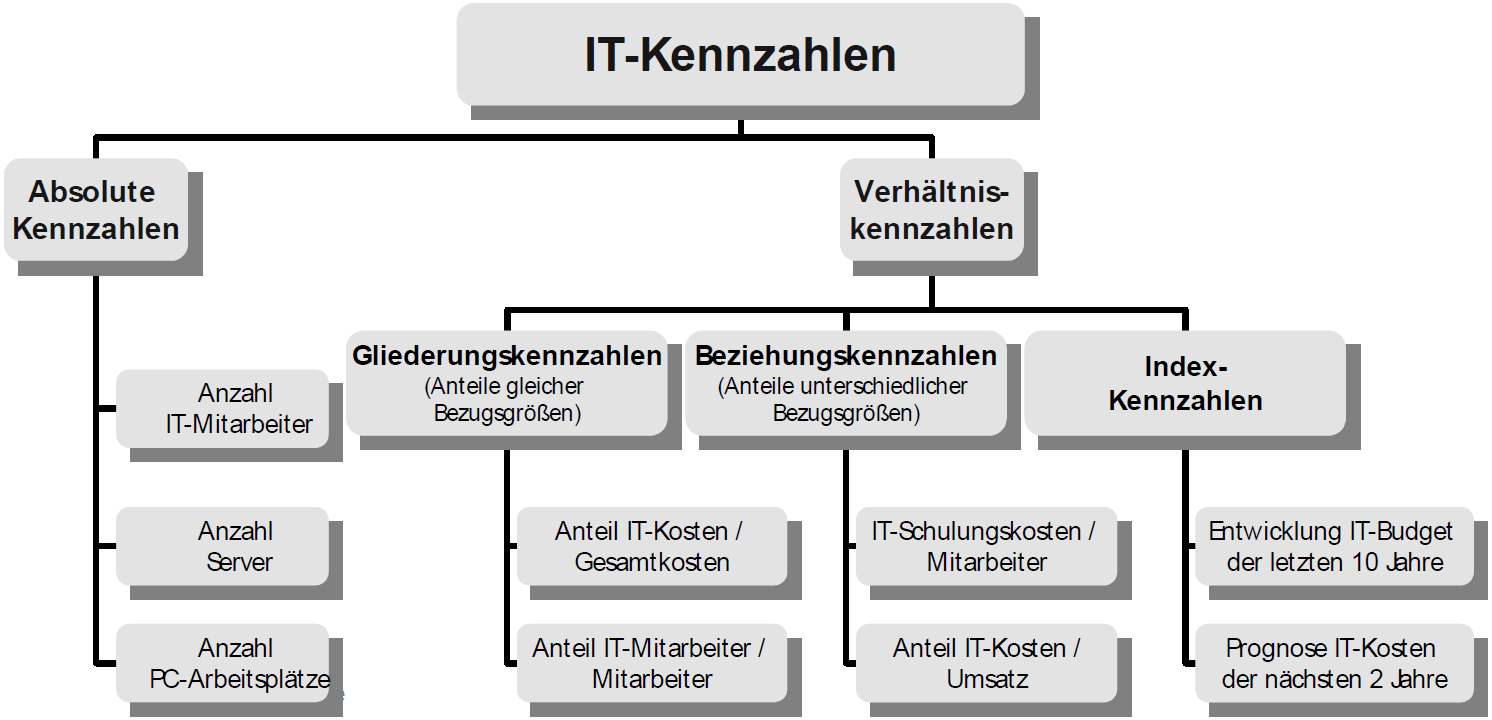
\includegraphics[width=0.8\textwidth]{BilderAllgemein/it_kennzahlen.PNG}
	\caption{Übersicht IT Kennzahlen \cite{Gadatsch10}}
	\label{img:uebersicht_it_kennzahlen}
\end{figure}

Abb. \ref{img:uebersicht_it_kennzahlen} zeigt die Struktur von IT Kennzahlen, welche sich in absolute Kennzahlen und Verhältniskennzahlen aufteilen. Verhältniskennzahlen splitten sich wiederum in Gliederungskennzahlen, Beziehungskennzahlen und Indexkennzahlen. \\
Im Vergleich zu den absoluten Kennzahlen, welche bereits aus messbaren, numerischen Größen bestehen, wird bei den Verhältniskennzahlen der Wert durch Berechnung ermittelt. \\
Bei den Gliederungskennzahlen wird eine Teilgröße in Beziehung zu einer Gesamtgröße gesetzt. Ein Beispiel ist der Anteil an IT-Kosten im Vergleich zu den Gesamtkosten. \\
Die Beziehungskennzahl gilt als aussagekräftigste Kennzahl. Für die Berechnung werden Größen, welche in einem sachlogischen Zusammenhang stehen, in Verbindung gesetzt. Als Beispiel dienen die IT-Schulungskosten / Mitarbeiter. \\
Indexkennzahlen werden verwendet, um eine zeitliche Veränderung von gleichartigen Kennzahlen darzustellen. Für die Berechnung wird ein Basiswert zu einem Basiszeitpunkt gleich 100 gesetzt. Eine zu einem späteren Zeitpunkt erfasste Größe stellt dann die Entwicklung als Vergleichswert dar. Die Prognose der IT-Kosten für die nächsten zwei Jahre ist ein Beispiel der Indexkennzahlen \cite{Gadatsch10} \cite{Jung07}.

Die folgende Liste zählt die wichtigsten Analysebereiche für IT Kennzahlen inklusive Beispielen für die jeweiligen Bereiche auf:

\begin{itemize}[noitemsep]
\item Wirtschaftlichkeit $\rightarrow$ Welche Vorteile bringt die Durchführung eines IT Projektes? Welche Kosten sind damit verbunden? Werden Gewinne erzielt? Wird der Bekanntheitsgrad des Unternehmens gesteigert?
\item Innovationsgrad der IT $\rightarrow$ Lohnt sich ein Upgrade der IT Hardware? Soll die veraltete IT Hardware weiter betrieben werden?
\item Prozessqualität $\rightarrow$ Welchen Einfluss hat die IT auf den Geschäftsprozess? 
\item Ressourcenauslastung in der IT $\rightarrow$ Welche Ausbildung haben die IT Mitarbeiter? Ist die Nutzung der Mitarbeiter effizient? Wie viele IT Mitarbeiter sind aktiv \cite{Gadatsch10}?
\end{itemize}

\subsection{IT-Kennzahlensysteme}

Aufgrund der geringen Aussagekraft von einzelnen, isolierten IT Kennzahlen werden im IT Management IT-Kennzahlensysteme verwendet. Diese Kennzahlensysteme stellen einzelne IT Kennzahlen in einen logischen Zusammenhang und unterstützen somit ein fachgerechtes IT Controlling \cite{Gadatsch10}. 

Es existieren mehrere IT-Kennzahlensysteme, welche im Laufe der Zeit von unterschiedlichen Firmen entwickelt wurden. \\
Das SVD-Kennzahlensystem, entwickelt 1980 von der Schweizerischen Vereinigung für Datenverarbeitung, ist hauptsächlich auf die Planung, Kontrolle und Steuerung der Wirtschaftlichkeit von IT-Systemen ausgelegt. Im Speziellen wird hierzu das Management, der Benutzer und die Informationsverarbeitung berücksichtigt \cite{Gadatsch10}.

\begin{figure}[h!]
	\centering
	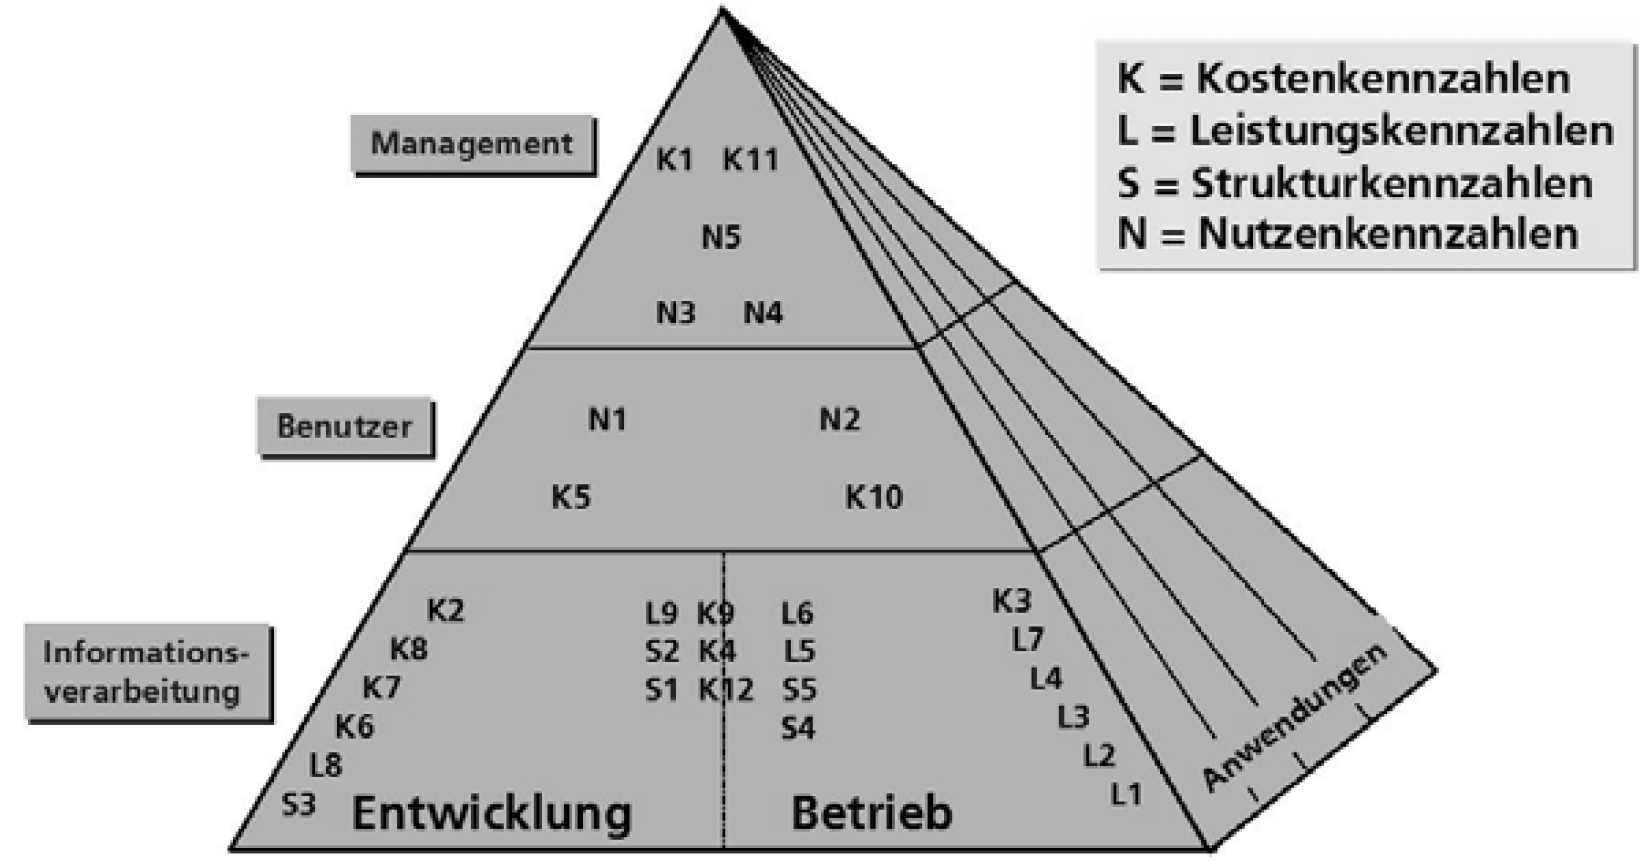
\includegraphics[width=0.8\textwidth]{BilderAllgemein/svd_kennzahlensystem.PNG}
	\caption{SVD Kennzahlensystem \cite{Biethahn00}}
	\label{img:svd_kennzahlensystem}
\end{figure}

Abb. \ref{img:svd_kennzahlensystem} zeigt das SVD Kennzahlensystem. Es besteht aus 30 Kennzahlen, welche sich in die vier Gruppen Leistungs-, Kosten-, Struktur- und Nutzenkennzahlen unterteilen. Die Leistungs-, Kosten- und Strukturkennzahlen lassen sich aus dem internen Rechnungswesen und der Personalwirtschaft generieren. Die Nutzenkennzahlen geben an, wie sinnvoll die Nutzung der IT im Vergleich zu keiner Nutzung der IT ist \cite{Gadatsch10}.

Im folgenden sind drei Kennzahlen ersichtlich, welche speziell im Rahmen dieser Bachelorarbeit relevant sind \cite{Gadatsch10}:

\textbf{L1 - Verfügbarkeit:}

$$Verfügbarkeit = \frac{Sollstunden - Ausfallstunden}{Sollstunden}$$

Die Verfügbarkeit definiert die Wahrscheinlichkeit, dass ein Objekt (Komponente oder System) zu einem bestimmten Zeitpunkt eine bestimmte Leistung erbringt. Sie wird in mehrere Klassen unterteilt, wobei zwischen einfacher Verfügbarkeit mit 99,5\%, Hochverfügbarkeit mit 99,999\% und Non-Stop Verfügbarkeit mit 100\% unterschieden wird. Um einen Ausfall zu verhindern gilt es Datenverarbeitungssysteme und Kommunikationswege stets redundant auszuführen \cite{Availability}.

Unter Anbetracht der obigen Formel, umgeändert auf Minuten, bedeutet eine Hochverfügbarkeit eine erlaubte Ausfallzeit von 5,256 Minuten in einem Zeitraum von einem Jahr: 

$Ausfallzeit = Sollzeit - (Verfügbarkeit * Sollzeit) = (365 * 24 * 60) - (0.99999 * 365 * 24 * 60) = 5,256$

\textbf{L2 - Zuverlässigkeit:}

$$Zuverlässigkeit = \frac{Sollstunden}{Anzahl\;der\;Ausfälle}$$

Die Zuverlässigkeit beschreibt die Wahrscheinlichkeit, ein Objekt zu einem bestimmten Zeitpunkt in einem funktionierenden Zustand vorzufinden. Die mittlere Zeit \ac{MTBF}, welche zwischen zwei Fehlern eines Objektes vergeht, wird als Maß der Zuverlässigkeit bezeichnet. \\
Je länger diese Zeit ist, desto zuverlässiger ist das Objekt. In der Theorie kann diese Zeit gegen unendlich gehen, in der Praxis jedoch nicht, da die Zeit durch die Lebensdauer begrenzt ist. Mit zunehmender \ac{MTBF} nimmt jedoch die Anzahl an Fehlern innerhalb eines definierten Zeitraums ab \cite{Eberlin14}. 

\begin{figure}[h!]
	\centering
	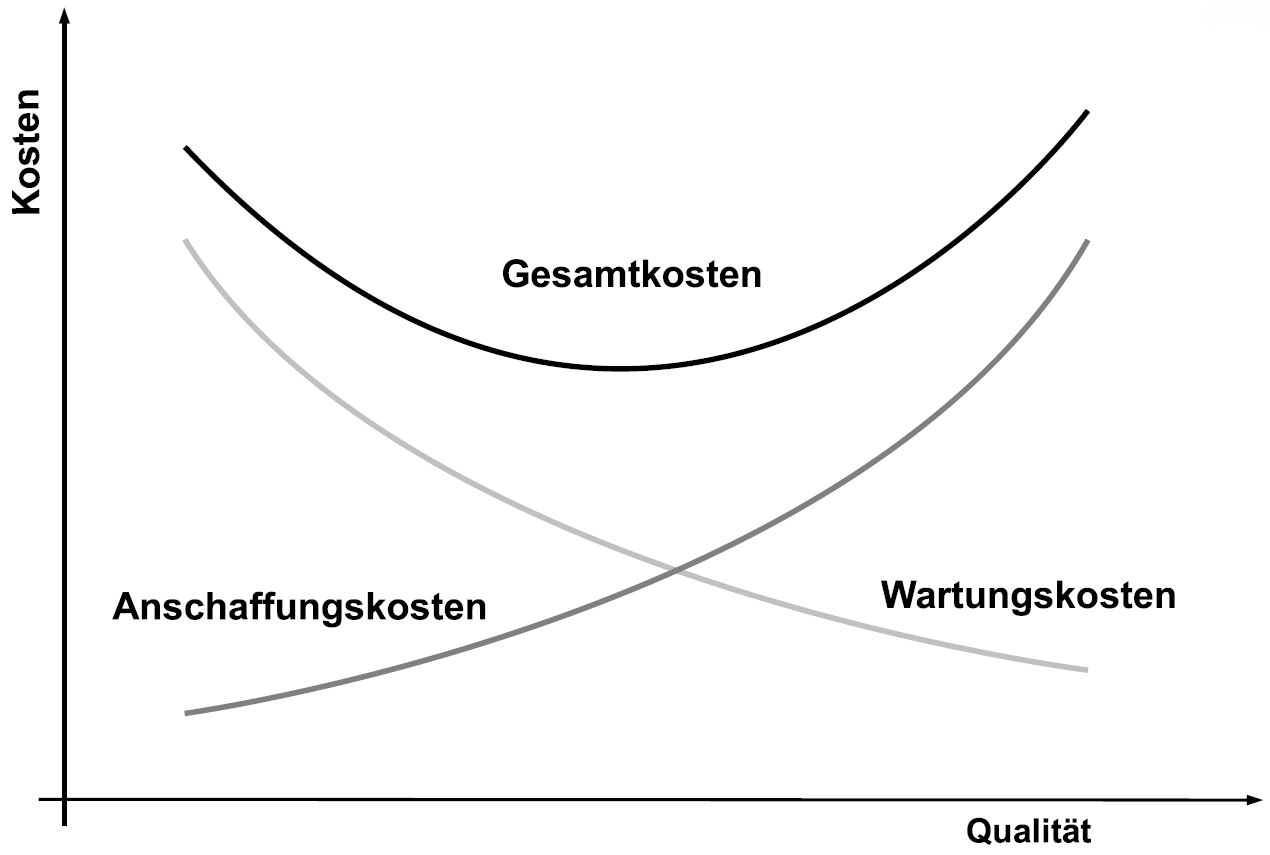
\includegraphics[width=0.6\textwidth]{BilderAllgemein/kosten_der_zuverlaessigkeit.PNG}
	\caption{Kosten der Zuverlässigkeit \cite{Eberlin14}}
	\label{img:kosten_der_zuverlaessigkeit}
\end{figure}

Abb. \ref{img:kosten_der_zuverlaessigkeit} zeigt einen typischen Verlauf von Anschaffungskosten, Wartungskosten und den daraus resultierenden Gesamtkosten. Die Kosten der Zuverlässigkeit sind beim Schnittpunkt zwischen Anschaffungskosten und Gesamtkosten minimal. Es gilt somit, Kosten und Qualität gegeneinander abzuwägen um Gesamtkosten zu sparen \cite{Eberlin14}.

\textbf{L3 - Durchschnittliche Reparaturzeit:}

$$Durchschnittliche\;Reperaturzeit = \frac{Reparaturzeit}{Anzahl\;von\;Reparaturen}$$

Die durchschnittliche Reparaturzeit ist Teil der Instandhaltbarkeit. Sie gibt an, wie schnell und mit welchem Aufwand ein Objekt nach einem Fehler wieder in den operativen Zustand gebracht werden kann \cite{Maintainability}.

Laut DIN IEC 60300-3-10 ist die Instandhaltbarkeit folgendermaßen definiert:

\begin{quote}
Fähigkeit einer Einheit, unter gegebenen Anwendungsbedingungen in einem Zustand erhalten bzw. in ihn zurückversetzt werden zu können, in dem sie eine geforderte Funktion erfüllen kann, wobei vorausgesetzt wird, dass die Instandhaltung unter den gegebenen Bedingungen mit den vorgeschriebenen Verfahren und Hilfsmitteln durchgeführt wird. \upshape \cite[S. 9]{Din04}.
\end{quote}